\chapter{Universal and Modular Jastrow Factors for the Transcorrelated Method}
\label{chap:universal}

The contents of this chapter are planned to be expanded for a future publication. Some contents may be repeated there.

\section{Introduction}

So far, the \gls{TC} methods we have discussed had one major bottleneck in common: the optimisation of the Jastrow factor. While VMC in itself does not scale unfavourably, the fact that we need so many VMC cycles in order to properly optimise for TC (see \autoref{chap:opt}) results in a significant computational cost. For large systems, this can become the prohibitive step in the workflow.

Here we explore some alternative avenues to construct Jastrow factors for use in the transcorrelated method. In particular, we consider constructing ``universal'' Jastrow factors that do not need any optimisation. These have already been introduced in the literature,\supercite{fournaisNonIsotropic2007,fournaisSharp2005,tewSecond2008,szenesStriking2024} and are constructed to satisfy cusp conditions. We will also construct Jastrow factors from those optimised for atomic systems. That is, we optimise the Jastrow factor for the atom, and use the same Jastrow factor for molecules (so that the molecular Jastrow is the sum of atomic Jastrows). In effect, this would allow us to compile sophisticated atomic Jastrow factors that may be stored in a database for easy retrieval when considering larger systems, without any optimisation. We also consider keeping some components of these Jastrows fixed, while optimising other elements as a ``molecular correction'' to the atomic Jastrow factor.

These updated workflows represent significant improvements in the scalability and ease of use for TC methods, while arguably being more conceptually satisfying by making the Jastrow factors more general.

\section{Theory}

In this chapter, we study various choices of Jastrow factors to avoid the need for lengthy optimisation. These may be divided into two broad categories: universal Jastrow factors and atomic Jastrow factors.

\subsection{Universal Jastrow Factors}

A universal form for the Jastrow factor has already been presented by Fournais \emph{et al} in 2005,\supercite{fournaisSharp2005} and has occasionally made further appearances in the literature.\supercite{tewSecond2008,szenesStriking2024} The key advantage to using these is that we require no optimisation at all, while key disadvantages are that we must be careful about cut off functions, and we do not have as much flexibility so we cannot tailor the Jastrow factor to e.g. excited states.

The universal form of the Jastrow, which we shall dub the ``Fournais-Jastrow'' factor is given by\supercite{fournaisSharp2005,fournaisNonIsotropic2007}
\begin{equation}
    \label{eq:fournais-full}
    J = -\sum_I\sum_i Z_Ir_{iI} + \frac 12\sum_{i<j}r_{ij} + \frac{2-\pi}{6\pi}\sum_I\sum_{i<j}Z_I\bm r_{iI}\cdot \bm r_{jI}\ln(r_{iI}^2+r_{jI}^2),
\end{equation}
where, as usual, upper case indices denote the nucleus, and lower case indices represent electrons. The first term resolves the electron-nucleus cusps, the second term resolves the electron-electron cusps, and finally the last term resolves electron-electron-nucleus cusps. However, these terms are unbounded, and indeed are valid only close to coalescence points. For this reason, we introduce cutoff functions on each term.

Using the form of the cutoff functions used in previous chapters, that is $t(r,L) = (1-r/L)^3\Theta(r-L)$, we find unreasonable energies even for extremely small cutoffs. For example, with this form of cutoff with the electron-nucleus and electron-electron terms, and $L=0.1$ Bohr, we get a reference energy of $-246.604$ for N$_2$ with the \avtz basis set, whereas the \gls{HEAT} result is known to be $-109.5425$.\supercite{fellerSurvey2008}

Thus, we instead use gaussian cutoffs, which are smooth but still decay rapidly. Our Jastrow factor therefore becomes
\begin{align}
    \label{eq:fournais-full-cutoffs}
    J &= -\sum_I\sum_i Z_Ir_{iI}\e^{-r_{iI}^2/L_{en}^2} + \frac 12\sum_{i<j}r_{ij}\e^{-r_{ij}^2/L_{ee}^2} \nonumber \\
    &\quad + \frac{2-\pi}{6\pi}\sum_I\sum_{i<j}Z_I\bm r_{iI}\cdot \bm r_{jI}\ln(r_{iI}^2+r_{jI}^2)\e^{-r_{iI}^2/L_{een}^2}\e^{-r_{jI}^2/L_{een}^2},
\end{align}
where $L_{ee}, L_{en}, L_{een}$ are cutoff parameters. For this study, we take $L\mathdef L_{ee} = L_{en} = L_{een}$, and consider three variants of equation \ref{eq:fournais-full-cutoffs}:
\begin{itemize}
    \item The full Fournais-Jastrow factor, as in equation \ref{eq:fournais-full-cutoffs}.
    \item Neglecting the electron-electron-nucleus term and resolving the electron-nucleus cusp using the approach described in \autoref{chap:opt} (instead of via the $r_{iI}$ terms). We'll dub this the $ee+en$-Jastrow.
    \item Neglecting both the electron-electron-nucleus and electron-nucleus terms. This has already been studied in the context of TC-DMRG,\supercite{szenesStriking2024} though the choice of cutoffs may result in uncontrollably nonvariational energies. This is the simplest form, containing only $r_{ij}$ terms, and we dub it the ``$ee$-Jastrow''.
\end{itemize}

Consider again the nitrogen molecule at equilibrium. We treat the result from \gls{HEAT}\supercite{fellerSurvey2008} as the exact nonrelativistic ground state energy, and so this is as a lower bound for the lowest eigenvalue of $\htc$ for the various Jastrow factors. For each of the three choices above, there is only one parameter, $L$. For the Fournais-Jastrow factor, we find that the reference xTC-energy with a cutoff of $L=0.1$ Bohr at \avtz is $-115.122$ Hartree, which is below the HEAT result. This may be due to numerical issues from the complexity of this Jastrow factor form, or it may indicate a more complex relationship between the TC energy and the cutoff $L$. However, since this is such a small cutoff, the TC and non-TC energies should be roughly equal. Therefore, for simplicity, we exclude the Fournais-Jastrow factor from this study and consider only the $ee$- and $ee+en$-Jastrow factors.

The energy of N$_2$ and N with the \avtz basis set for the $ee$- and $ee+en$-Jastrow factors are shown in figure \ref{fig:fournais-cutoff-n2}. Shown are three non-TC energies: the non-TC (RHF) reference energy, the non-TC-FCIQMC energy, and the HEAT (effectively \gls{CBS}) energy. Plotted as a function of $L$ are three TC energies, the xTC (RHF) reference energy, the xTC-MP2 energy, and the xTC-FCIQMC energy. For small $L$, we expect the non-TC- and xTC- reference and FCIQMC energies to coincide, which they approximately do. In contrast, for large $L$ we expect the energies to become unstable, as we start to include spurious long-range correlation. However, it is worth noting that according to these plots, ``long-range'' is already at $\approx 0.4$ Bohr, as the energies are all below the HEAT result. In every case, $L=0.3$ Bohr is shown to result in energies above that of HEAT but below that of non-TC. We therefore use $L=0.3$ Bohr as our ``universal'' cutoff for these Jastrow factors.

\begin{figure}[h!]
    \centering
    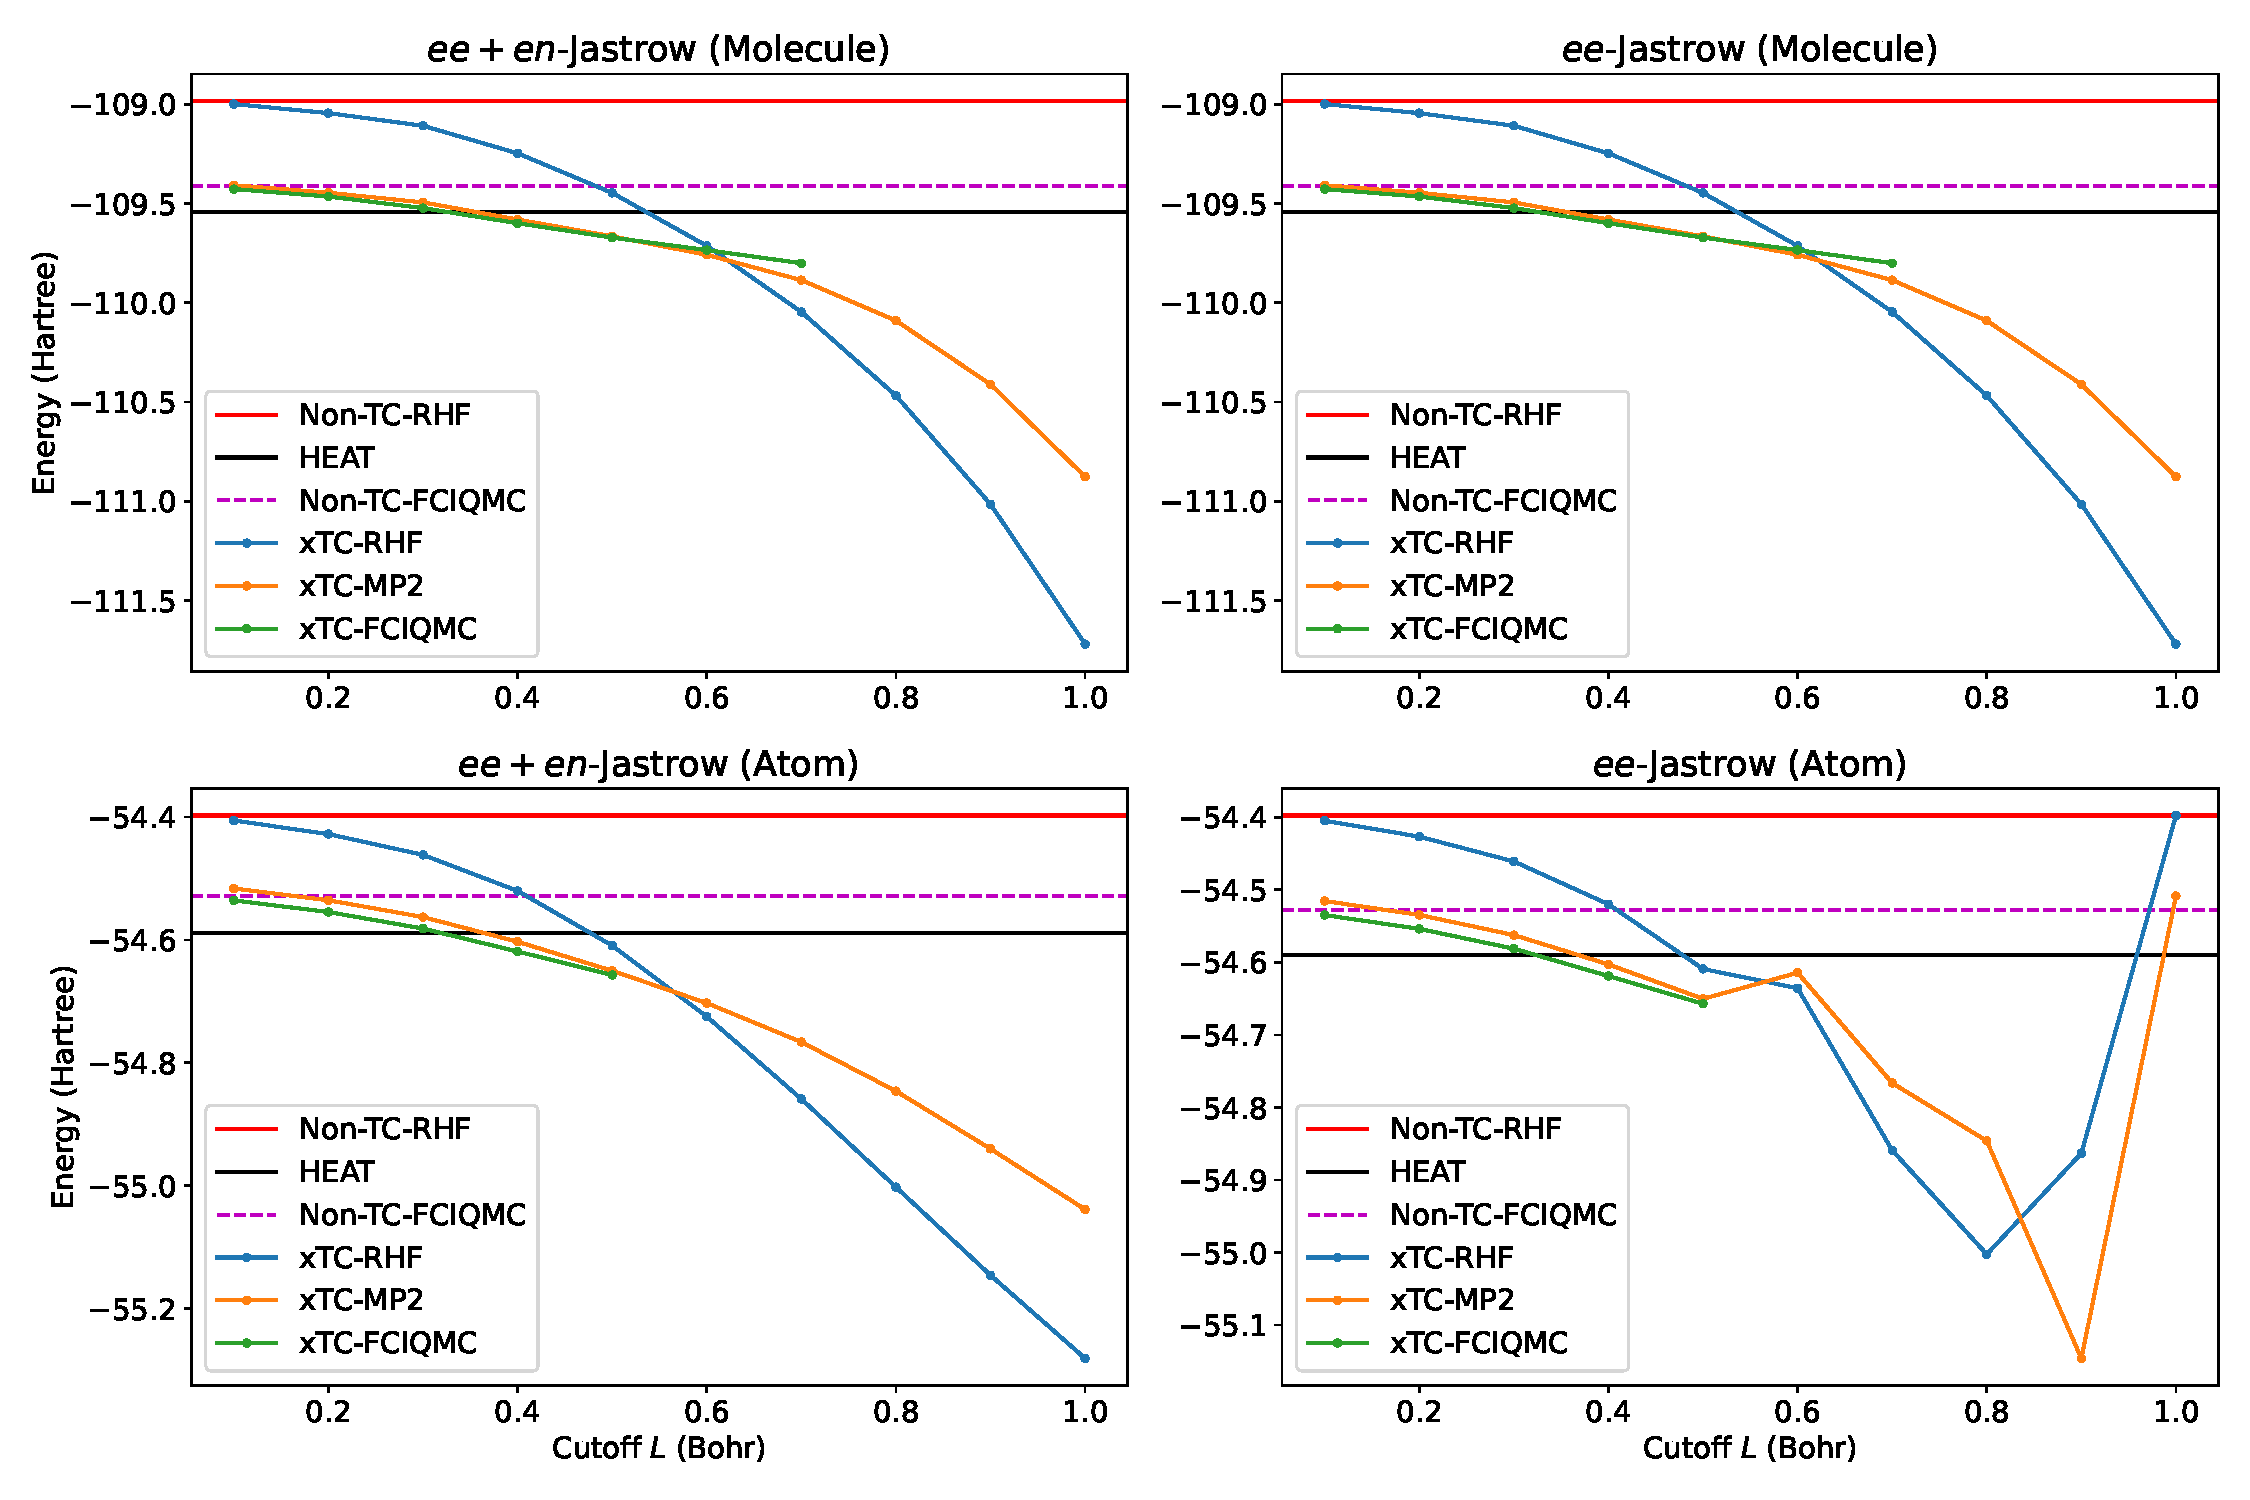
\includegraphics[width=\textwidth]{figures/universal/cutoffs_combined}
    \caption{Energy estimates for the nitrogen molecule (top panel) and atom (bottom panel) as a function of a cutoff parameter $L$ for the $ee+en$- (left panel) and $ee$-Jastrow (right panel) factors. The non-TC reference (RHF) energies are represented by a horizontal red line, the HEAT result by a horizontal black line, and the non-TC-FCIQMC by a dashed line. Since HEAT is a \gls{CBS}-extrapolated method, we wish for our TC energies to be above this value, while we also wish to improve upon the non-TC-FCIQMC energy. We therefore take the value of $L$ that leads to sensible energies (i.e. above the HEAT result), which is $L=0.3$ for all four plots. Large- and small-$L$ limits behave as expected, with the former giving nonsensical results and the former approximating the non-TC results in that basis set. All calculations were performed with the \avtz basis set. Missing xTC-FCIQMC points are due to numerical instability caused by a positive correlation energy. In practice, these may be resolved by setting a positive shift, but these results are anyway undesirable.}
    \label{fig:fournais-cutoff-n2}
\end{figure}

Since TC amounts to a similarity transformation, and any similarity transformation exactly preserves the eigenspectrum in the CBS limit, we know that this undesirable behaviour must be a basis set effect. Moreover, since the effects of these Jastrow factors are extremely localised near the nuclei, we might expect core-valence basis functions to aid in the TC energies. Figure \ref{fig:basis-vs-cutoff} shows the effect of adding core functions to the basis set for the $ee+en$-Jastrow factor. We see that the core functions increase the (positive) correlation energies to bring it closer to the CBS limit, as does increasing the size (cardinal number) of the basis set. However, even cc-pCVQZ is not enough to bring the xTC-MP2 energy above the HEAT result for cutoff values above 0.4 Bohr. This suggests a very strong basis set effect, and merits further studies.

\begin{figure}[h!]
    \centering
    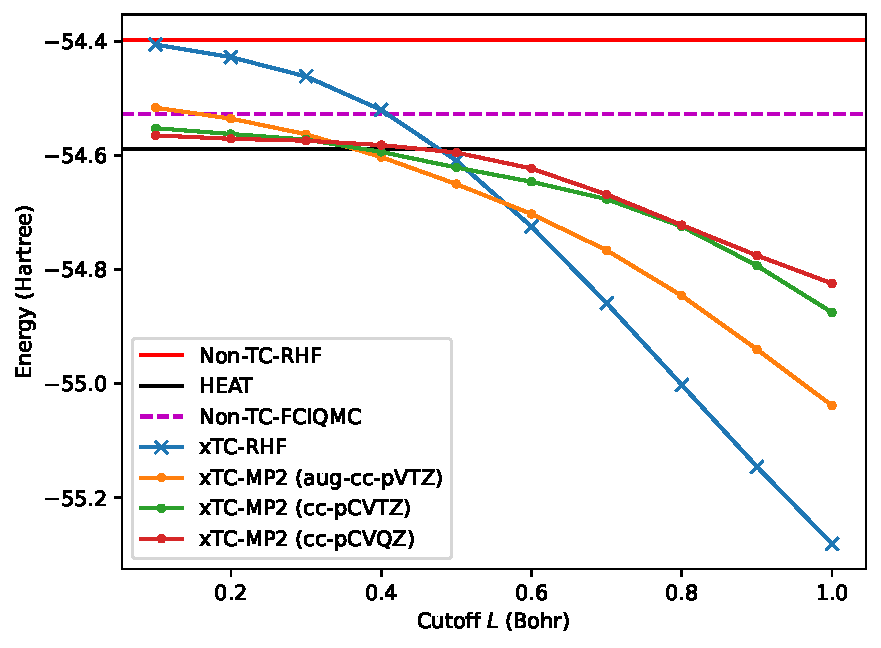
\includegraphics[width=0.8\textwidth]{figures/universal/cutoffs_basis.pdf}
    \caption{MP2 energies as a function of the cutoff $L$ for the $ee+en$-Jastrow factor. The xTC-RHF values are roughly the same for each basis set shown. Adding core functions significantly improves the curve to be closer to the HEAT result, resulting in larger (positive) correlation energies. Increasing the cardinal number of the basis set also improves the curve, but the effect is less pronounced. Nevertheless, these results indicate a strong basis set effect in the cutoff, particularly for core functions.
    Adding diffuse functions have negligible effects on the curve (e.g. xTC-MP2 curves for aug-cc-pCVTZ and cc-pCVTZ roughly coincide).}
    \label{fig:basis-vs-cutoff}
\end{figure}

% \todo{also comment on Fournais}

\subsection{Atomic Jastrow Factors}

Another approach we consider in reducing the need for optimisation is to optimise Jastrow factors for atomic systems and then reuse them in the molecular context. This can be considered a natural TC extension of starting with atomic orbitals for molecules. The key advantage here is flexibility while the key disadvantages include the need to optimise for the atoms, and the need to make a choice for the form of the Jastrow factor. In principle, we could produce a database of sophisticated atomic Jastrow factors that can then be queried to construct Jastrow factors for molecules or periodic systems. We use the Jastrow forms considered earlier in this dissertation, \begin{equation}
    \label{eq:jastrow-3}
    J = \sum_{i<j}^Nv(r_{ij}) + \sum_i^N\sum_I^{N_A}\chi(r_{iI}) + \sum_{i<j}^N\sum_I^{N_A}f(r_{ij}, r_{iI}, r_{jI}),
\end{equation}
with
\begin{equation}
    \label{eq:dtn-jastrow-ee-3}
    v(r_{ij})    = t(r_{ij},L_v)
                    \sum_{k} a_k r_{ij}^k ,
\end{equation}
\begin{equation}
    \label{eq:dtn-jastrow-en-3}
    \chi(r_{iI}) = t(r_{iI},L_\chi)
    \sum_{k} b_k r_{iI}^k ,
\end{equation}
\begin{equation}
    \label{eq:dtn-jastrow-een-3}
    f(r_{ij}, r_{i}, r_{j}) = t(r_{iI},L_f) t(r_{jI},L_f)
    \sum_{k,l,m} c_{klm}
    r_{ij}^k r_{iI}^l r_{jI}^m ,
\end{equation}
and the same cutoff functions $t(r,L) = (1-r/L)^3
\Theta(r-L)$. However, we do not want to include long-range (with respect to the nucleus) correlation in the atomic Jastrow factors, since this may bias the molecular calculations. We therefore use $L_v=L_\chi=1.0$ Bohr and $L_{v}=4.5$ Bohr. We consider the following variants:
\begin{itemize}
    \item The Jastrow factor is kept constant for the molecule, i.e. we simply use the atomic Jastrow factors as they are. We refer to these as simply ``atomic'' Jastrow factors.
    % \item We optimise the atomic Jastrow factor only with terms involving the nucleus, i.e. electron-nucleus and electron-electron-nucleus terms. The electron-electron part is then added to the atomic Jastrow factor and optimised for the target system (e.g. a molecule) with the electron-nucleus and electron-electron-nucleus term fixed at the values determined for the atom. We refer to these as ``atomic$(n)+ee$'' Jastrow factors. As we shall see, these ``over-correlates'' the the electrons in the atoms compared to the \todo{}
    \item We optimise the atomic Jastrow factor using all terms. Then, when calculating molecules, we fix all terms involving nuclei and re-optimise the electron-electron terms. We refer to these as ``atomic$+ee$'' Jastrow factors.
\end{itemize}

We find these to yield results above HEAT and therefore do not concern ourselves with a cutoff analysis as in the case of the universal Jastrow factors.

\section{Results}

\subsection{Computational Details}

We revisit the nitrogen binding curve from \autoref{chap:binding} as a stress test for our Jastrow factors, as well as the atomisation of the molecules N$_2$, C$_2$, O$_2$, and CN from \autoref{chap:opt}. As before, we compare the results of the different choices of Jastrow factors against experiment\supercite{leroyAccurate2006} and the atomisation energies to HEAT.\supercite{fellerSurvey2008} The binding curve is calculated with the \avtz basis set, while the atomisation energies are calculated with the \avxz{$X$} basis sets for $X=\text{D},\text{T},\text{Q}$.

For the multideterminantal optimisation, we use a small FCIQMC calculation as it was found to perform particularly well in \autoref{chap:binding}, while keeping the orbitals consistent with the atom. Non-TC HF and CASCI calculations were performed using \pyscf,\supercite{sunPySCF2018} VMC optimisation was performed using \casino,\supercite{needsVariational2020} FCIQMC calculations using \neci,\supercite{gutherNECI2020} and MRCI-F12 calculations for comparison using \molpro.\supercite{wernerMOLPRO,wernerMolpro2012,wernerMolproQuantumChemistry2020}


\subsection{Atomisation Energies}

For the atomisation energies, we focus on the $ee+en$ and atomic$+ee$ Jastrow factors, as these are the most ``complete'' of each category of Jastrow factors presented here.
\todo{...}
\todo{include both ways of optimising the ee terms from the atomic, and show that we should also optimise it in the atom so that the en and een terms don't compensate for it missing}


\begin{table}[htbp]
    \centering
    \begin{tabular}{c|c|ccc||c}
    System & Jastrow & \vdz & \vtz & \vqz & \gls{CBS}\supercite{fellerSurvey2008,bytautasCorrelation2005} \\
    \hline
    \multirow{4}{*}{N$_2$} & Non-TC & -109.2809 & -109.4014 & -109.4653 & \multirow{4}{*}{-109.5425} \\
      & Full TC & -109.4727 & -109.5312 & -109.4528 &  \\
      & $ee+en$ & -109.4125 & -109.5141 & \textbf{-109.5580} &  \\
      & Atomic+$ee$ & -109.4364 & \red{-109.5167} & \red{-109.5405} &  \\
    \hline
    \multirow{4}{*}{C$_2$} & Non-TC & -75.7320 & -75.8094 & -75.8578 & \multirow{4}{*}{-75.9240} \\
    & Full TC & -75.8844 & -75.9197 & -75.9272 &  \\
    & $ee+en$ & -75.8153 & -75.8823 & \red{-75.9213} &  \\
    & Atomic+$ee$ & -75.8567 & \red{-75.9080} & \red{-75.9249} &  \\
    \hline
    \multirow{4}{*}{O$_2$} & Non-TC & -149.9915 & -150.1554 & -150.2362 & \multirow{4}{*}{-150.3273} \\
    & Full TC & -150.2216 & -150.3078 & -150.3244 &  \\
    & $ee+en$ & -150.1972 & -150.3243 & \textbf{-150.3662} &  \\
    & Atomic+$ee$ & \todo{} & \todo{} & \todo{} &  \\
    \hline
    \multirow{4}{*}{CN} & Non-TC & -92.4970 & -92.5954 & -92.6517 & \multirow{4}{*}{-92.7232} \\
    & Full TC & -92.6671 & -92.7152 & -92.7247 &  \\
    & $ee+en$ & -92.6039 & -92.6872 & \textbf{-92.7281} & \\
    & Atomic+$ee$ & -92.6331 & -92.6992 & \red{-92.7204} & \\
    \hline\hline
    \multirow{4}{*}{N} & Non-TC & -54.4801 & -54.5252 & -54.5535 & \multirow{4}{*}{-54.5893} \\
    & Full TC &  -54.5622 & -54.5842 & -54.5896  \\
    & $ee+en$ & -54.5425 & -54.5792 & \textbf{-54.5986} & \\
    & Atomic+$ee$ & -54.5477 & -54.5786 & -54.5890 & \\
    \hline
    \multirow{4}{*}{C} & Non-TC & -37.7619 & -37.7900 & -37.8126 & \multirow{4}{*}{-37.8450} \\
    & Full TC & -37.8293 & -37.8427 & -37.8459 & \\
    & $ee+en$ & -37.8020 & -37.8256 & -37.8437 &  \\
    & Atomic+$ee$ & -37.8193 & -37.8374 & -37.8451 &  \\
    \hline
    \multirow{4}{*}{O} & Non-TC & -74.9117 & -74.9853 & -75.0236 & \multirow{4}{*}{-75.0674} \\
    & Full TC & -75.0226 & -75.0572 & -75.0665 &  \\
    & $ee+en$ & -75.0123 & -75.0686 & \textbf{-75.0882} &  \\
    & Atomic+$ee$ & -74.9986 & -75.0514 & -75.0657 &  \\
    \end{tabular}
    \caption{\todo{absolute energies, to compare esp to full TC}
    \todo{mention that full TC also has larger cutoffs! It is from a different paper!! also explains why the atoms have different energies}
    \todo{comparison against optimisation chapter}
    \todo{boldface means nonvariational}
    \todo{red means not yet converged NECI calculation}
    }
    \label{tbl:universal-absE}
\end{table}

\begin{table}[htbp]
    \centering
    \begin{tabular}{c|c|ccc||c}
    Molecule & Jastrow & \vdz & \vtz & \vqz & \gls{CBS}\supercite{fellerSurvey2008} \\
    \hline
    \multirow{4}{*}{N$_2$} & Non-TC & \todo{} & \todo{} & \todo{} & \multirow{4}{*}{\todo{}} \\
      & Full TC & \todo{} & \todo{} & \todo{} &  \\
      & $ee+en$ & \todo{} & \todo{} & \todo{} &  \\
      & Atomic+$ee$ & \todo{} & \todo{} & \todo{} &  \\
    \hline
    \multirow{4}{*}{C$_2$} & Non-TC & \todo{} & \todo{} & \todo{} & \multirow{4}{*}{\todo{}} \\
    & Full TC & \todo{} & \todo{} & \todo{} &  \\
    & $ee+en$ & \todo{} & \todo{} & \todo{} &  \\
    & Atomic+$ee$ & \todo{} & \todo{} & \todo{} &  \\
    \hline
    \multirow{4}{*}{O$_2$} & Non-TC & \todo{} & \todo{} & \todo{} & \multirow{4}{*}{\todo{}} \\
    & Full TC & \todo{} & \todo{} & \todo{} &  \\
    & $ee+en$ & \todo{} & \todo{} & \todo{} &  \\
    & Atomic+$ee$ & \todo{} & \todo{} & \todo{} &  \\
    \hline
    \multirow{4}{*}{CN} & Non-TC & \todo{} & \todo{} & \todo{} & \multirow{4}{*}{\todo{}} \\
    & Full TC & \todo{} & \todo{} & \todo{} &  \\
    & $ee+en$ & \todo{} & \todo{} & \todo{} & \\
    & Atomic+$ee$ & \todo{} & \todo{} & \todo{} & \\
    \end{tabular}
    \caption{\todo{atomisation energies}}
    \label{tbl:universal-atomisation}
\end{table}


\begin{figure}[htbp]
    \centering
    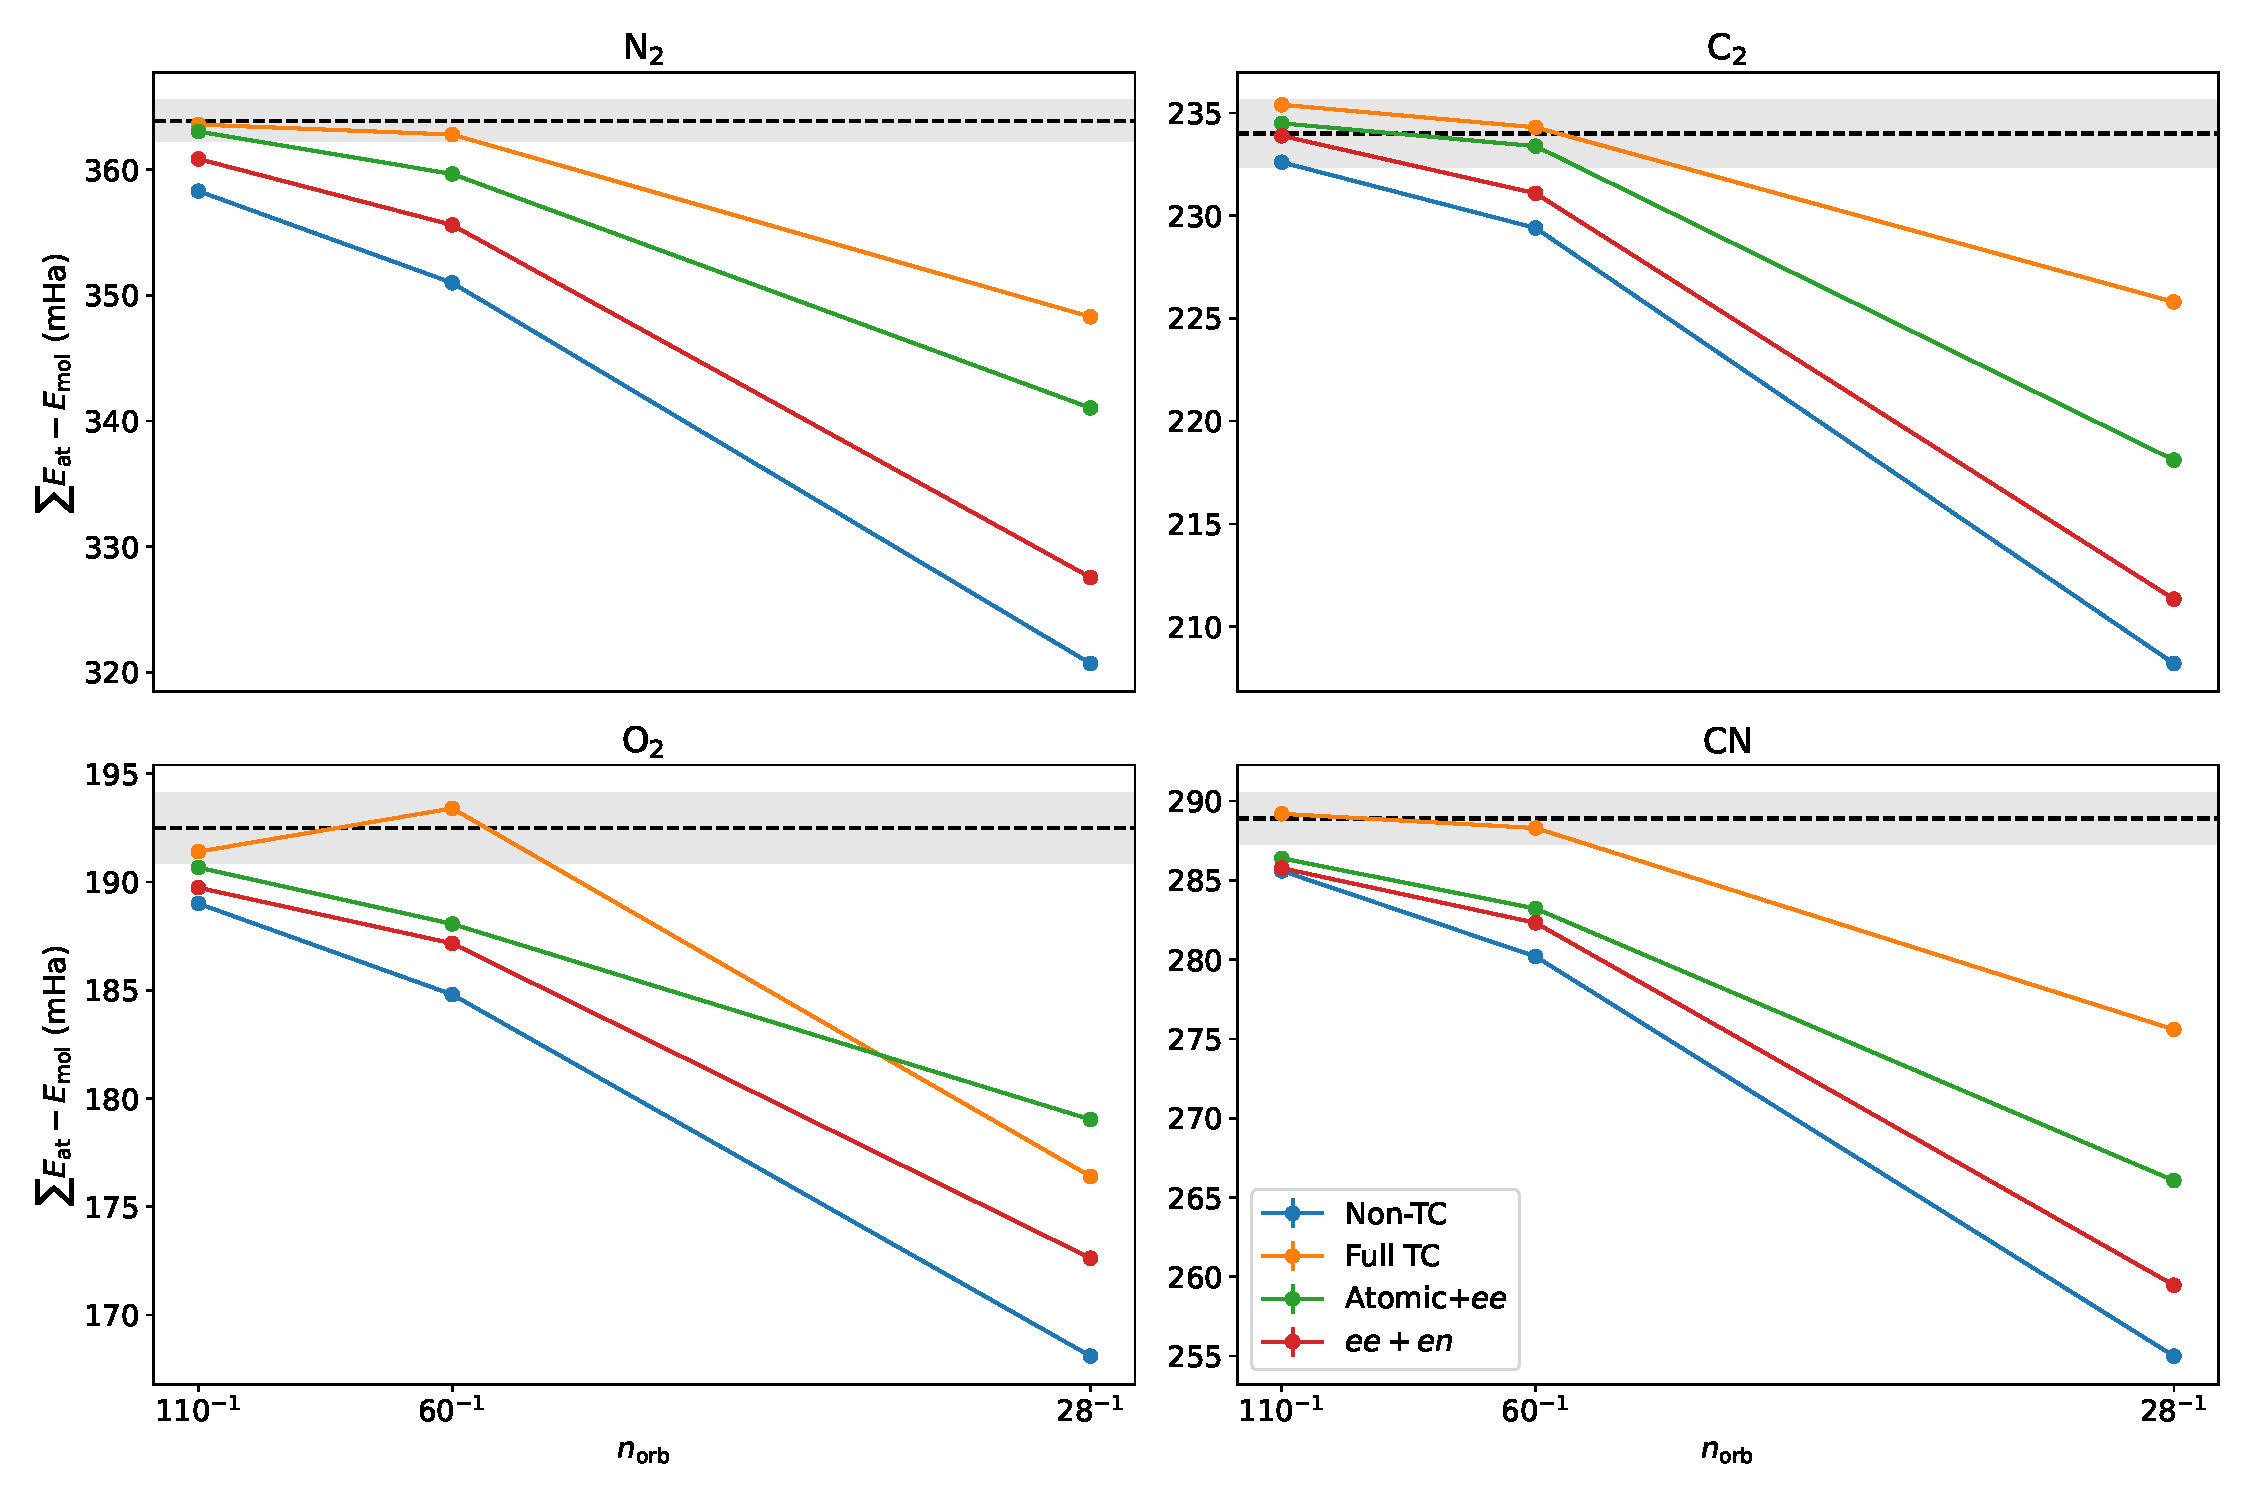
\includegraphics[width=\textwidth]{figures/universal/atomisation_energies}
    \caption{\todo{atomisation energies wrt number of orbitals}
    \todo{vtz and vqz calculations are not converged!}}
    \label{fig:universal-atomisation}
\end{figure}

% \todo{?absolute energies plot?}



\subsection{Binding Curves}

Here we report the N$_2$ binding curve with the \avtz basis set for the various choices of Jastrow factors. Values for the interatomic distance range between $1.92$ and $10$ Bohr. The Jastrow factors used were the atomic Jastrow factor, the atomic Jastrow factor with electron-electron terms optimised for the molecule (using a RHF or FCIQMC ansatz), the $ee$- and $ee+en$-Jastrow factors. The energy values relative to experiment (normalised such that $10$ Bohr is $0$) is shown in figure \ref{fig:binding-universal-experiment}. The FCIQMC-Jastrow (i.e. multideterminant ansatz with all terms optimised) curve from \autoref{chap:binding} is also shown for comparison.

\todo{...}

\begin{figure}[htbp]
    \centering
    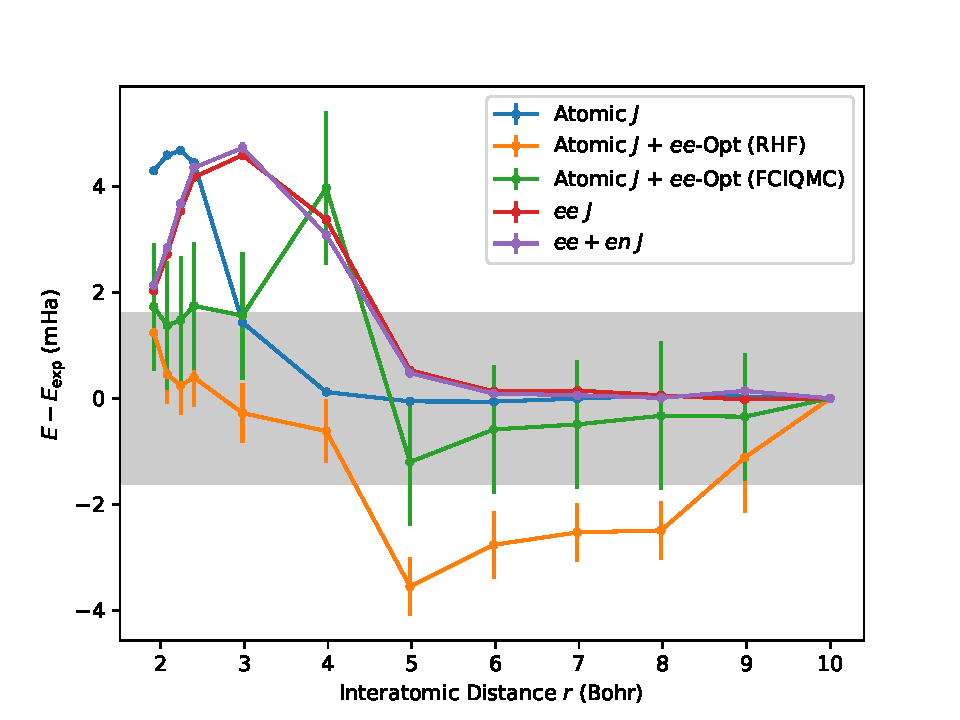
\includegraphics[width=\textwidth]{figures/universal/residuals}
    \caption{The binding curves relative to a fit to experimental data\supercite{leroyAccurate2006} for the N$_2$ binding curve, calculated in the \avtz basis for various Jastrow factor forms. All curves are normalised such that the value at $10$ Bohr is $0$. The grey shaded area denotes a region of $\pm 1.6$ mHa (chemical accuracy). For reference, the multideterminantal FCIQMC-Jastrow from \autoref{chap:binding} is shown in brown (with diamonds). Both universal Jastrow forms ($ee$ and $ee+en$, denoting with only electron-electron or with both electron-electron and electron-nucleus terms, respectively) stay above the experimental result, and are indeed very close to each other. The atomic Jastrow factors, whether not optimised for the molecule (atomic $J$), or containing $ee$ terms optimised for the molecule (RHF or FCIQMC as the $\Phi$ ansatz) have a less smooth behaviour, but are generally closer to the experimental result. \todo{converge these and update the caption: this data is preliminary}}
    \label{fig:binding-universal-experiment}
\end{figure}

\todo{...}

\begin{figure}[htbp]
    \centering
    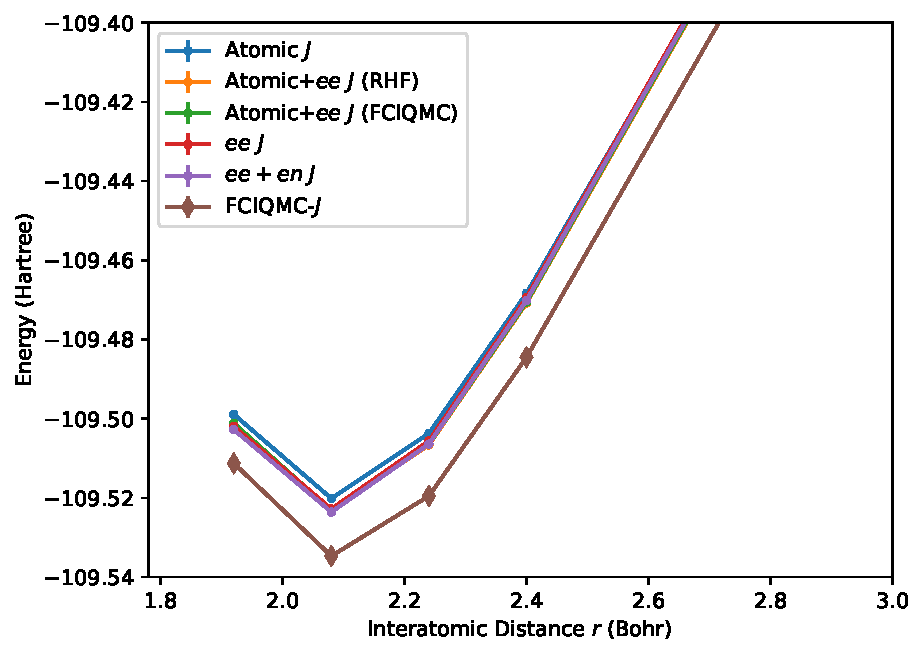
\includegraphics[width=0.8\textwidth]{figures/universal/n2_avtz_min}
    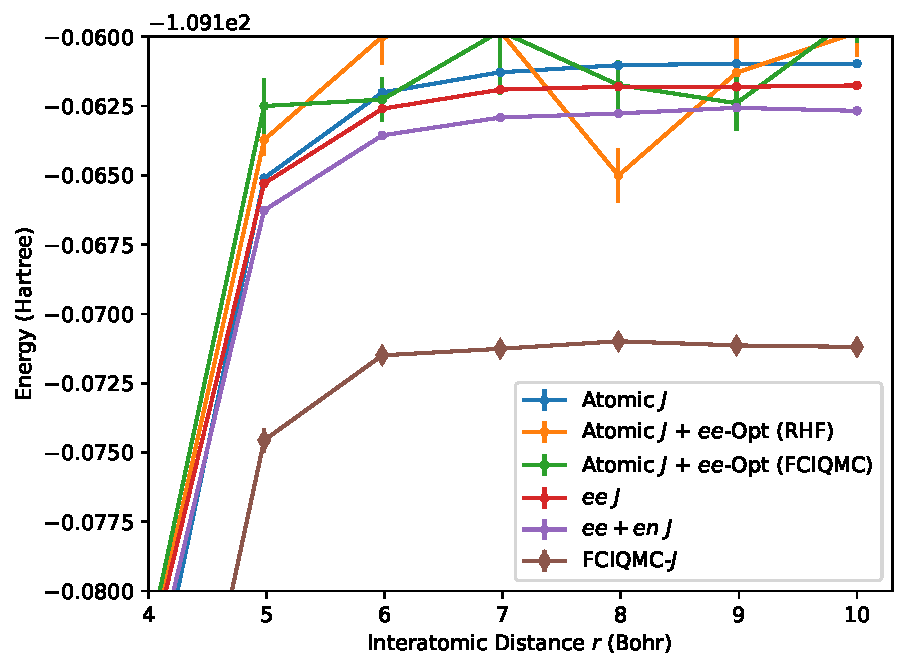
\includegraphics[width=0.8\textwidth]{figures/universal/n2_avtz_diss}
    \caption{Zoomed in views of the binding N$_2$ binding curves for the various Jastrow factor choices. All forms give qualitatively correct binding curves. Included for comparison is the FCIQMC-Jastrow from \autoref{chap:binding}, which was shown to be good both at equilibrium and dissociation. Compared to this, the binding curves for both universal Jastrow forms are shifted up, as well as for the atomic Jastrow factor without further optimisation. However, when we use the atomic Jastrow factor with the electron-electron terms optimised for the molecule, we get a curve that is very close to the FCIQMC-Jastrow, particularly when using a multideterminal (FCIQMC) expansion. \todo{converge these and update the caption: this data is preliminary. I expect (hope) the weird behaviour for the ee-opt RHF curve at 10 Bohr will go away}}
    \label{eq:binding-universal-zoom}
\end{figure}

\todo{size consistency discussion, atomisation energy using dissociated limit}

\begin{table}[!h]
    \centering
    \begin{tabular}{c|c}
        Jastrow Factor & $\sum E_\mathrm{atom} - E_\mathrm{molecule}(r=10)$ (mHa) \\
        \hline
        Atomic &  \\
        Atomic+$ee$ (SD) &  \\
        Atomic+$ee$ (MD) & \\
        $ee$ & \\
        $ee+en$ & \\
        \bottomrule
        % Non-TC & -3.9(1) \\
        MRCI-D-F12 & -0.9
    \end{tabular}
    \caption{
        \todo{}
    }
    \label{tbl:size-consistency-uni}
\end{table}

\begin{table}[!h]
    \centering
        \begin{tabular}{c|c}
            Jastrow Factor & Atomisation Energy (mHa) \\
            \hline
            Atomic &  \\
            Atomic+$ee$ (SD) &  \\
            Atomic+$ee$ (MD) & \\
            $ee$ & \\
            $ee+en$ & \\
            \bottomrule
            MRCI-D-F12 & 359.5 \\
            HEAT\supercite{fellerSurvey2008} & 363.9 \\
            Experiment\supercite{leroyAccurate2006} & 363.7
        \end{tabular}
    \caption{\todo{...}}
    \label{tbl:binding-atomisation-energies-uni}
\end{table}

\section{Conclusion and Outlook}
\todo{mention the shortcoming of not being able to target specific states like the previous methodology (except for quasi-atomic)}
\todo{mention the fournais/universal form does not faithfully capture long-range correlation}
\todo{mention possibility of combining methods, also using the orbital cusp correction for the Fournais factor}
\todo{mention that with the small optimisation we introduce the possibility of targeting specific states, at least somewhat}
\todo{mention revisiting the universal Jastrow factors and the cutoffs more thoroughly}
\todo{...}
\todo{outlook: optimising $L$, using different cutoff functions}
\todo{ECPs with universal/atomic Jastrows to mitigate the effects from the core!}
\todo{a more sophisticated way of handling heterogeneous systems}

\todo{Also mention (maybe by then you even have data for) the Fournais Jastrow factor}
